\documentclass{report}[14pt]
\usepackage[a4paper,total={6.5in,8.5in}]{geometry}
\usepackage[main=spanish,english]{babel}
\usepackage{lmodern}
\usepackage{graphicx}   % para \includegraphics
\usepackage{subcaption} % define el entorno subfigure

\usepackage{float}           % [H]
\usepackage{placeins}        % \FloatBarrier
\usepackage{enumitem}
\usepackage{amsmath}
\usepackage{listings}
\usepackage{wrapfig}
\usepackage{svg}             % si realmente usas .svg → perfil Inkscape pdf_tex
\usepackage{booktabs}
%  Ajuste de floats global (opcional)
\setcounter{topnumber}{5}
\setcounter{bottomnumber}{5}
\setcounter{totalnumber}{10}
\renewcommand{\topfraction}{0.9}
\renewcommand{\bottomfraction}{0.9}
\renewcommand{\textfraction}{0.05}
\renewcommand{\floatpagefraction}{0.9}

\usepackage{listings}
\lstset{
  inputencoding=utf8,
  extendedchars=true,
  literate={á}{{\'a}}1 {é}{{\'e}}1 {í}{{\'i}}1 {ó}{{\'o}}1 {ú}{{\'u}}1 {ñ}{{\~n}}1
           {Á}{{\'A}}1 {É}{{\'E}}1 {Í}{{\'I}}1 {Ó}{{\'O}}1 {Ú}{{\'U}}1 {Ñ}{{\~N}}1
           {¿}{{?}}1 {¡}{{!}}1 {ü}{{\"u}}1 {Ü}{{\"U}}1,
  basicstyle=\ttfamily\small,
  columns=flexible,
  keepspaces=true,
  showspaces=false,   % <<< desactiva la visualización de espacios como "_"
  showstringspaces=false,
  frame=single,
  captionpos=b,
  breaklines=true
}

\usepackage{hyperref}
\usepackage{titlesec}

\usepackage[backend=biber,style=numeric]{biblatex}
\addbibresource{hola.bib}


% Configuración de márgenes
\renewcommand{\thesection}{\arabic{section}}
\renewcommand{\thesubsection}{\arabic{section}.\arabic{subsection}}



\begin{document}

% Portada
\begin{titlepage}
    \begin{center}
        \vspace*{\fill}  % Empieza a llenar desde arriba hasta que se centra
        
\includegraphics[width=10cm]{ceu.png}\\[1cm]
        \textbf{\LARGE Universidad CEU}\\[1.5cm]
        \textbf{\LARGE  Proyecto Aprendizaje Automático}\\[2cm]
         {\Large \textbf{Autores}: \par}
        {\Large Humberto Pérez De La Blanca Osta\par}
        {\Large Jaime Rodriguéz Del Portillo\par}
        {\Large Cristina Suaréz Limón\par}
        {\Large  Valentina Villalobos Padrino \par}
        \vspace*{\fill}  % Completa el espacio restante hasta centrar verticalmente
    \end{center}
\end{titlepage}

% Índice
\tableofcontents
\newpage

\chapter{Introducción}
El abandono escolar temprano constituye uno de los principales retos del sistema educativo, tanto en España como en otros países de la Unión Europea. Aunque en los últimos años, las cifras han mejorado, sigue siendo causa de gran preocupación, especialmente debido a su impacto en la empleabilidad, la inclusión social y la igualdad de oportunidades.

Según datos recientes del Ministerio de Educación, Formación Profesional y Deportes, en 2024 se sitúa en un 13\%, lo que supone una reducción del 0.7 puntos respecto al año anterior y una bajada de 8,9 puntos respecto con 2014. Esta mejora, aunque significativa, todavía se enfrenta a desigualdades de género (15,8\% en hombres frente a 10\% en mujeres) y factores estructurales que aún limitan la permanencia estudiantil, especialmente en los primeros años universitarios.

En este contexto, se vuelve imprescindible anticipar cuales son las barreras o condiciones que están contribuyendo al abandono. El presente trabajo emplea un conjunto de datos reales del Instituto Politécnico de Portalegre (Portugal), recogido en el momento de inscripción de los estudiantes y sin considerar su rendimiento posterior. El objetivo es construir modelos clasificadores que predigan el destino académico del estudiante —abandono, continuación o graduación— basándose únicamente en información disponible al inicio del curso. 

Para ello, se han definido cuatro enfoques de modelado, cada uno desarrollado por un miembro del equipo, con el objetivo de aportar perspectivas complementarias:

\begin{itemize}
    \item Se aplicará una regresión logística con enfoque interpretativo. Su objetivo es analizar qué variables están más fuertemente asociadas al abandono académico y facilitar la comprensión de sus causas.
    \item Se implementará un modelo de k-vecinos más cercanos, centrado en detectar patrones de similitud entre estudiantes para predecir el desenlace académico.
    \item Se entrenará un árbol de decisión que permite visualizar, tal y como su nombre lo indica, rutas de decisión e inferir reglas comprensibles para predecir si un estudiante continuará, abandonará o se graduará.
    \item Se diseñará una red neuronal simple, con el propósito de comparar el rendimiento con modelos clásicos y explorar su capacidad para captar relaciones lineales y patrones complejos.
\end{itemize}
 
A través del análisis comparativo de estos modelos, se busca determinar cuál de ellos ofrece mejores resultados en términos predictivos y cual proporciona mayor valor predictivo.  En consecuencia, con este proyecto se persigue mejorar la precisión de las predicciones y ofrecer una herramienta útil para la toma de decisión relacionada con la mejora de la permanencia y el éxito en la educación superior

\chapter{Análisis Exploratorio de los Datos}
Tras contextualizar el problema, se procede al análisis exploratorio del conjunto de datos, etapa fundamental e imprescindible en cualquier proyecto de Aprendizaje Automático. Esta primera fase tiene como objetivo:
\begin{itemize}
    \item Comprender la naturaleza y distribución de las variables.
    \item Detectar posibles errores, valores atípicos e inconsistencias.
    \item  Evaluar la calidad, representatividad y completitud de los datos.
    \item Tomar decisiones informadas relacionadas con la normalización y transformación de atributos.
\end{itemize}
El dataset utilizado contiene información académica, demográfica y social de más de 4.400 estudiantes, recogidas en el momento de la matrícula:
\section{Estructura y tipos de datos disponibles}
El dataset a utilizar contiene 4.424 registro, donde cada registro repersenta a un estudiantes matriculado en le universidad del estudio. Existen 37 columnas, las cuales se pueden clasificar de la siguiente manera:
\begin{itemize}
    \item \textbf{Variables categóricas binarias:} Toman valores de 0 a 1, representante atributos como el género, si tiene deudas con la institución, si dispone de beca, entre otras.
    \item \textbf{Variables categóricas multiclase:} Representan factores cualitativos con múltiples niveles. Algunas de ellas presentan alta cardinalidad, como ocupación del madre y de la madre, sus cualificaciones, la titulación en la que se matriculó, nacionalidad (será posteriormente transformada a una variable categórica binaria), entre otras.
    \item \textbf{Variables numéricas continuas:} Están codificadas como enteros o números de punto flotante, e incluyen aspectos cuantitativos relevantes como la edad, nota de admisión, asignaturas aprobadas e indicadores macronoéconomicos como la tasa de desempleo, la tasa de inflation y PIB.
    \item La variable objetivo \textbf{Target} es de tipo categórico con tres posibles valores: abandono (\textit{Dropout}), continúa activo (\textit{Enrolled}) y graduado (\textit{Graduated}).

\end{itemize}

\section{El tratamiento de valores faltantes, duplicados y outliers}
Una parte esencial del análisis exploratoria es evaluar la calidad de los datos, ya que errores pueden introducir sesgos e impedir la correcta generalización de los modelos.

\subsection{Datos faltantes:} 
Según la fuente de información de los datos \cite{noauthor_undated-nc} y tambien mediante el uso de la función \texttt{isnull().sum()} se verificó que no existen valores nulos en ninguna de las columnas del dataset, pudiendo así poder trabajar sin necesidad de imputación o eliminación de registros.

 
\subsection{Registros duplicados} Del mismo modo, mediante el uso del filtrado \texttt{duplicated()} se comprobó que inexistencia de datos duplicados, lo que confirma la integridad del conjunto de datos.

\subsection{Valores atípicos} Durante la fase de análisis exploratorio se llevó a cabo una exhaustiva revisión de los posibles valores atípicos (outliers) en las variables numéricas, tanto mediante visualizaciones (histogramas, boxplots y gráficos de dispersión) como con criterios estadísticos como el método del rango intercuartílico (IQR).

En el análisis resultante, se identificaron aproximadamente un 10\% de valores como atípicos, lo cual representa una proporción significativa. Sin embargo, tras una inspección detallada, se observó que:

\begin{itemize}
    \item Muchos de estos valores extremos son \textbf{coherentes y legítimos} dentro del dominio educativo (por ejemplo, estudiantes de mayor edad o calificaciones muy bajas).
    \item \textbf{Los patrones de dispersión de estos valores son consistentes} con el comportamiento general de la variable, y no se detectaron errores evidentes de codificación.
    \item Las distribuciones presentan comportamientos claramente diferenciados por clase (Dropout, Graduate, Enrolled), justificando que estas desviaciones no solo son reales, sino útiles para diferenciar perfiles estudiantiles.
    \item La eliminación o imputación agresiva de estos valores podría inducir sesgo o pérdida de variabilidad útil, reduciendo significativamente la riqueza y la capacidad predictiva del conjunto de datos en el entrenamiento de modelos.
    \item Las visualizaciones muestran distribuciones claramente sesgadas y heterogéneas según la clase, especialmente en variables como \textit{Curricular units approved} y \textit{Curricular units grade}, indicando que estos valores extremos aportan información predictiva valiosa.
\end{itemize}

Por tanto, se optó por una estrategia conservadora: \textbf{mantener los valores atípicos tal y como están en el dataset original}. Esta decisión está alineada con buenas prácticas cuando los valores atípicos tienen sentido en el contexto y no comprometen la estabilidad del modelo:


Se observa que las variables macroeconómicas no presentan datos atípicos, lo que es esperable debido a su poca variabilidad de los datos al hacer referencia a países, más no a los estudiantes en sí: 

\begin{figure}[H]
    \centering
    \begin{subfigure}[b]{0.32\textwidth}
        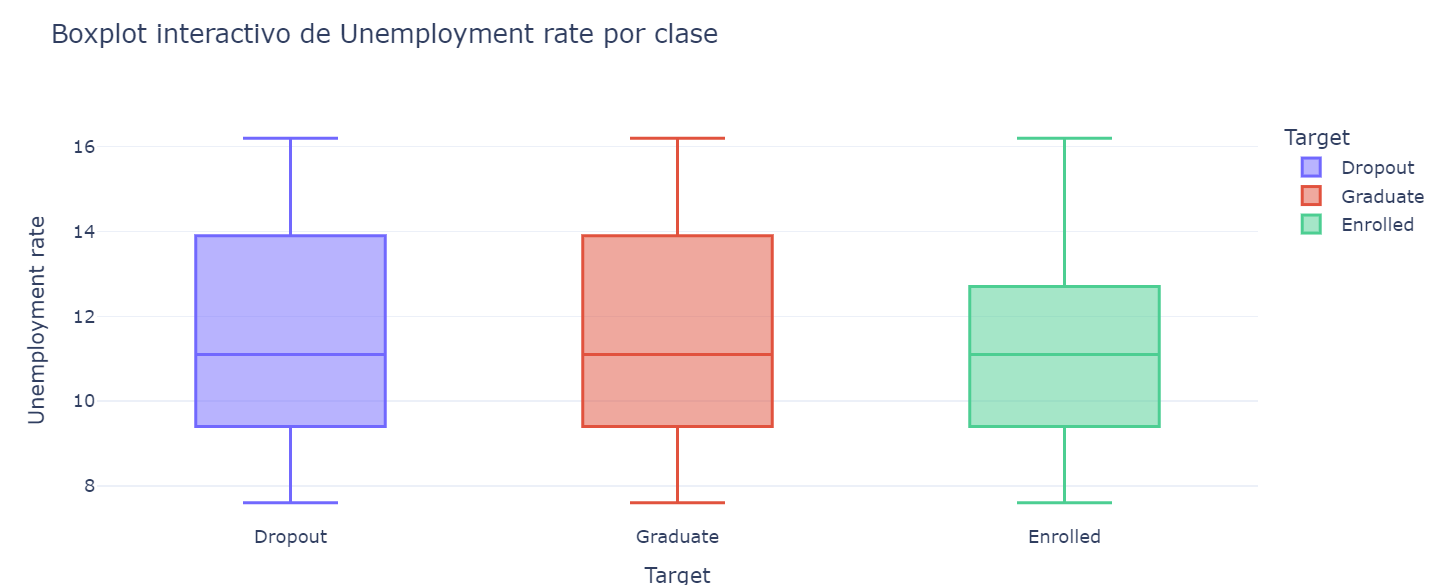
\includegraphics[width=\textwidth]{distribution_plotly/unemployment_rate.png}
        \caption{Unemployment rate}
    \end{subfigure}
    \hfill
    \begin{subfigure}[b]{0.32\textwidth}
        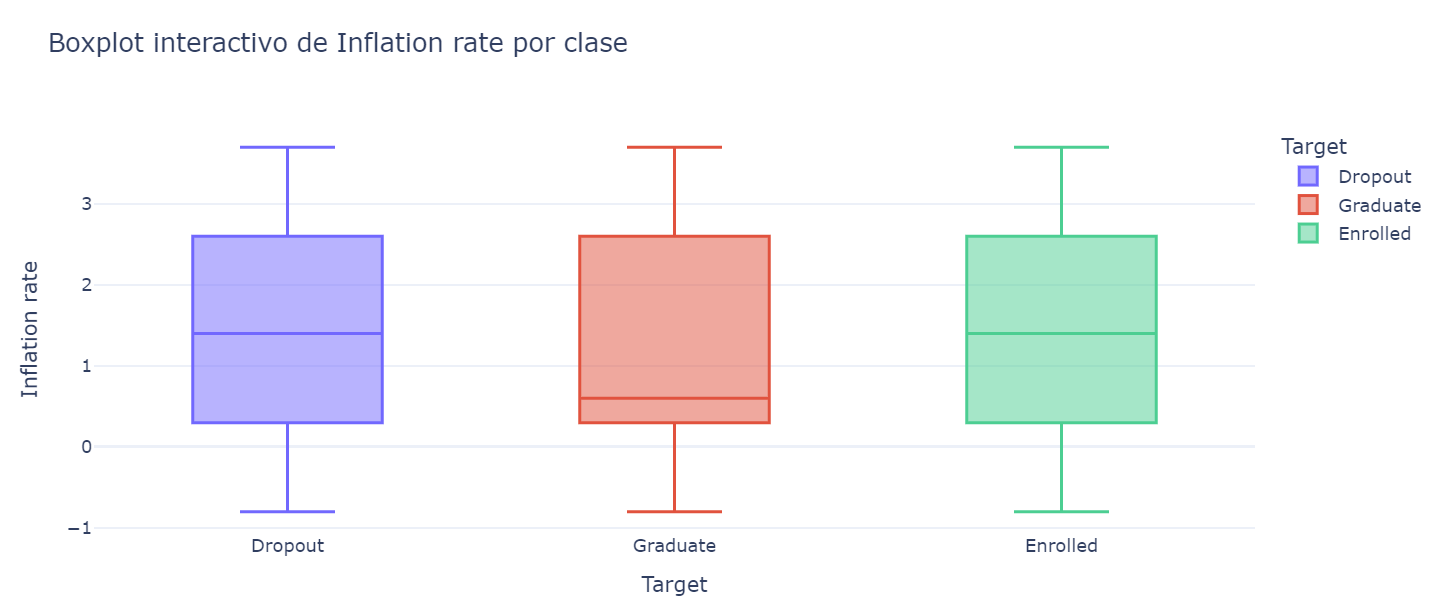
\includegraphics[width=\textwidth]{distribution_plotly/inflation_rate.png}
        \caption{Inflation rate}
    \end{subfigure}
    \hfill
    \begin{subfigure}[b]{0.32\textwidth}
        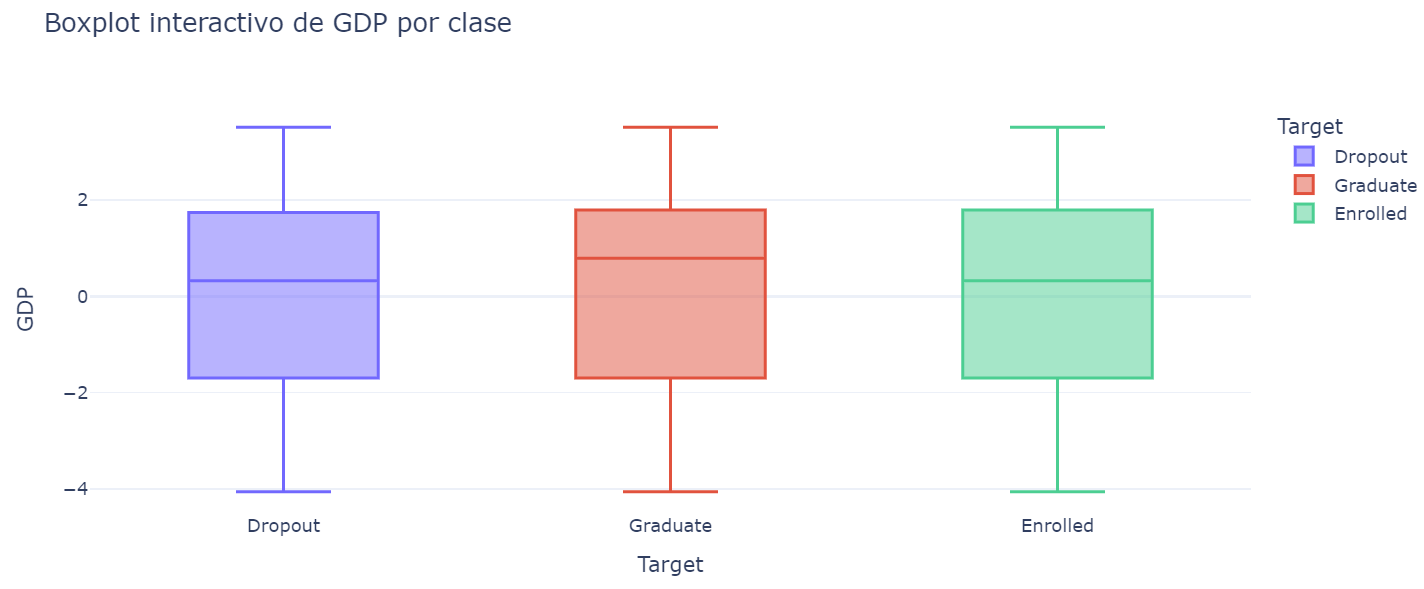
\includegraphics[width=\textwidth]{distribution_plotly/gdp.png}
        \caption{GDP}
    \end{subfigure}
    \caption{Distribución por clase de variables macroeconómicas}
    \label{fig:macroeconomicas}
\end{figure}


A continuación se verán casos concretos que respaldan dicha suposición:


\textbf{Variable Admission grade}

Sea la variable \textbf{\textit{Admission grade}}, la cual presenta la siguiente distribución y caja de bigotes separada por clases:
%\vspace{5cm}
\begin{figure}
    \centering
    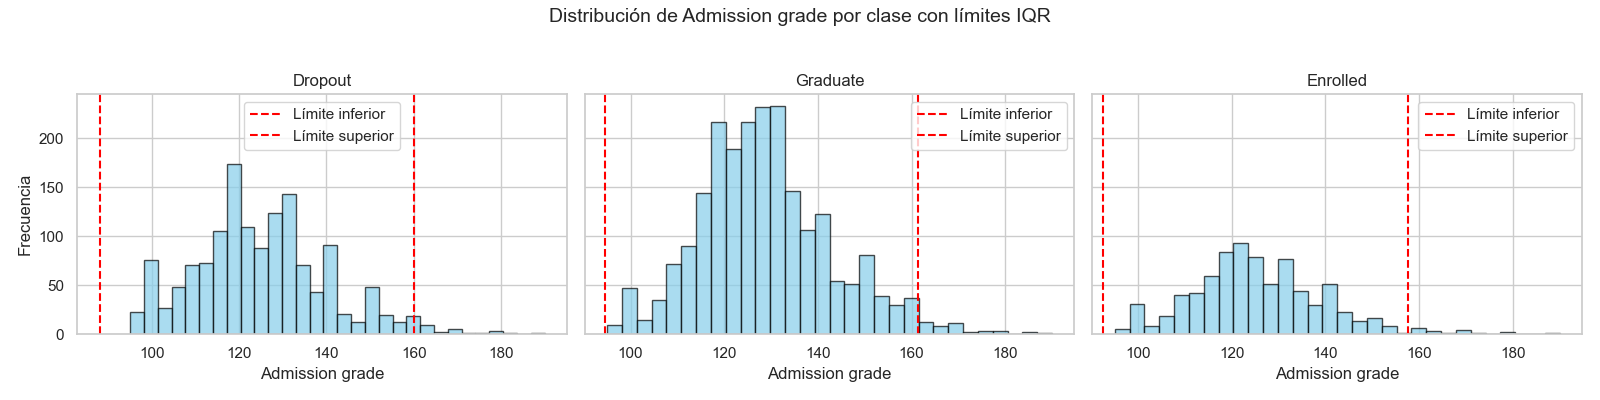
\includegraphics[width=0.75\linewidth]{distribution/Admission grade_distribution.png}
    \caption{Histograma separados por clases de la variable 'Admision Grade'}
    \label{fig:admisiongrade-label}
\end{figure}

\begin{figure}
    \centering
    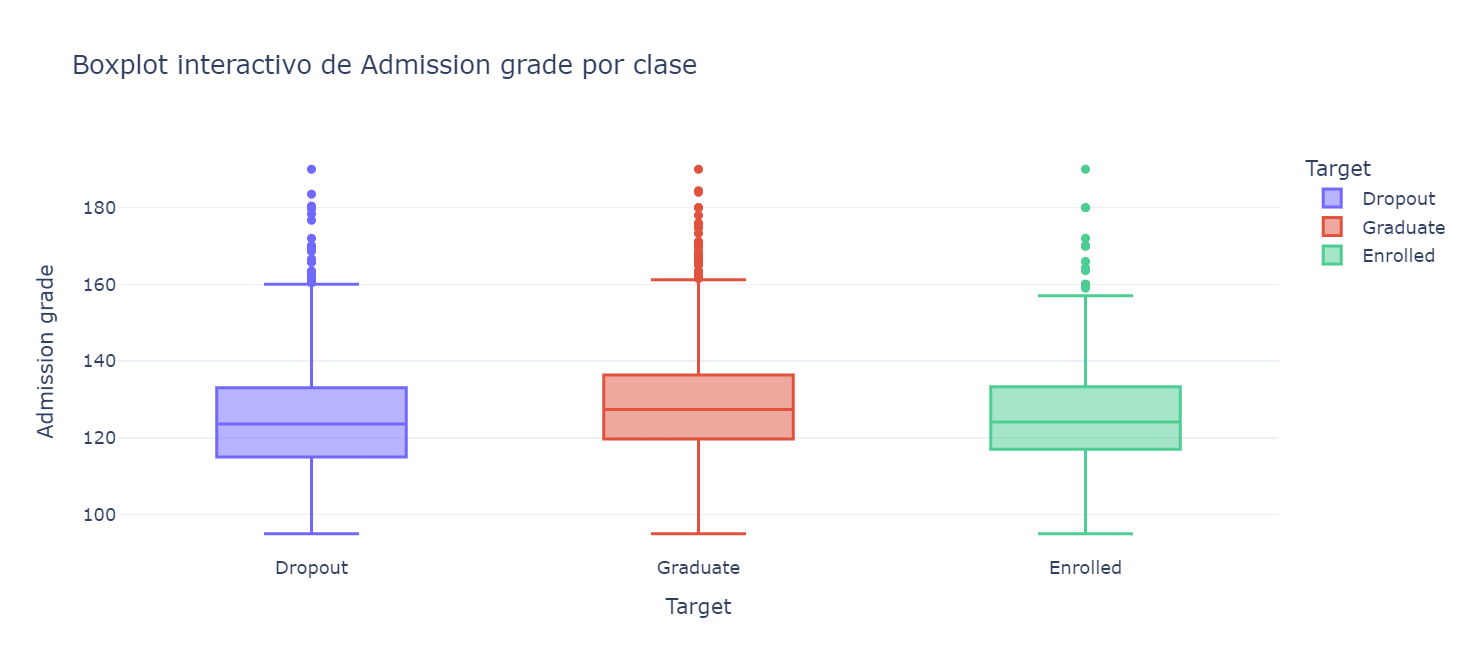
\includegraphics[width=0.75\linewidth]{distribution_plotly/admission_grade.png}
    \caption{Caja de bigotes separado por clases de la variable 'Admision Grade'}
    \label{fig:enter-label}
\end{figure}
\FloatBarrier
\textbf{Comentarios de las representaciones:}
\begin{itemize}
    \item La distribución en los tres casos es asimétrica negativa: hay una concentración alrededor de 120–130, con cola hacia la derecha.
    
    \item Los outliers por encima de 160 son pocos pero reales. Los estudiantes que se gradúan (Graduate) tienden a tener las notas de admisión más altas, con una mediana en torno a 130–135.
    
    \item Los que abandonan (Dropout) presentan una distribución más baja, aunque con outliers hacia arriba.
\end{itemize}
Confirmamos que la nota de admisión es predictiva del éxito académico.


\textbf{Variable Edad:} \\
La variable Edad presenta un comportamiento similar. Se observa que la edad media de un estudiante aumenta cuanto más riesgo tiene este de abandonar, esto se ve reflejado en los valores de los cuartiles y la distribución de la caja de bigotes de esta clase frente a las otras dos, cuya mayoría de datos están en el rango de los 18 a 25 frente al rango de 18 a 47 de la clase \textbf{\textit{'Dropout'}}. De lo anterior, se concluye que la edad esta claramente asociado con el abandona, reforzando su utilidad como variable predictiva relevante para los posteriores modelos.
\begin{figure}
    \centering
    \begin{subfigure}[b]{.75\linewidth}
        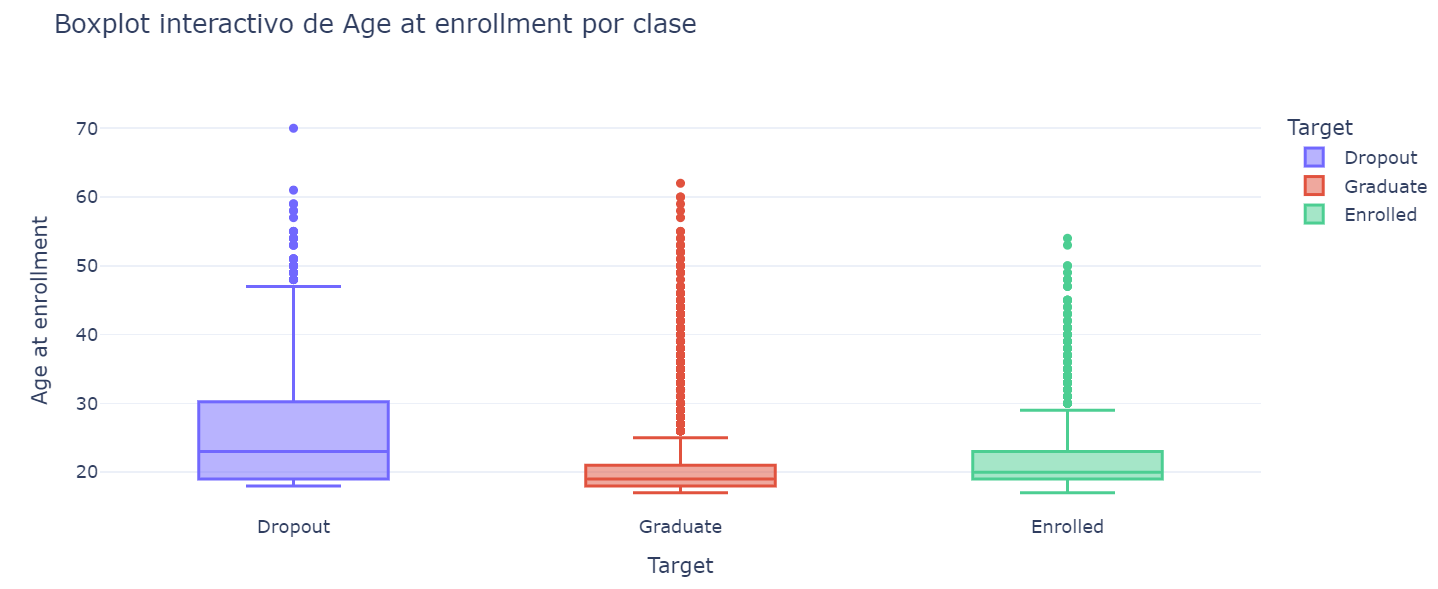
\includegraphics[width=0.75\linewidth]{distribution_plotly/age.png}
        \caption{Edad de entrada separada por clases}
        \label{fig:boxplot-age}
    \end{subfigure} \hfill
  \begin{subfigure}[b]{.75\linewidth}
        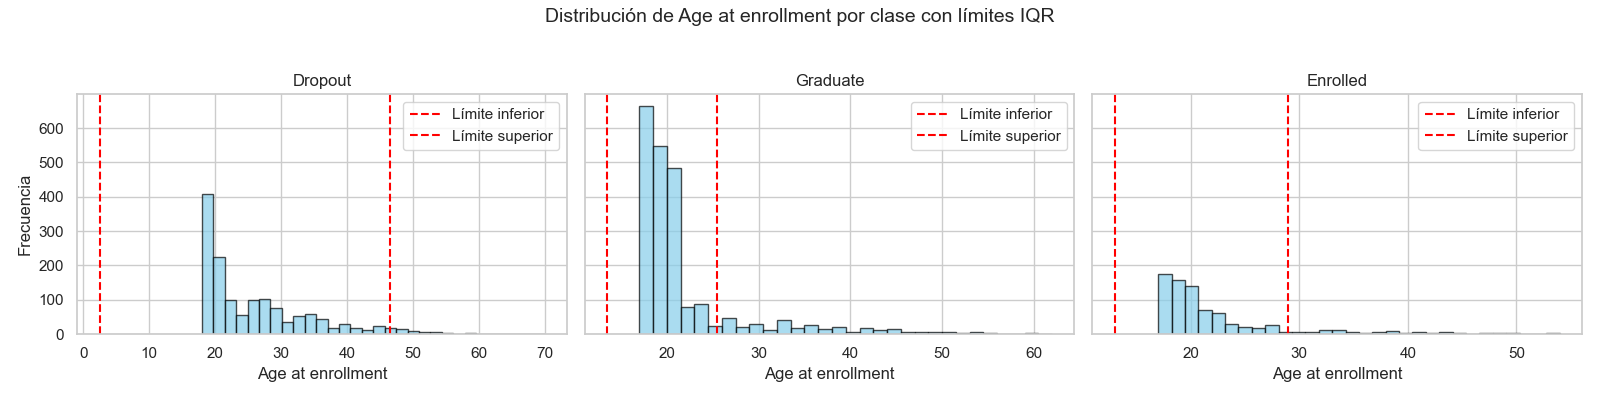
\includegraphics[width=0.75\linewidth]{distribution/Age at enrollment_distribution.png}
        \caption{Edad de entrada separada por clases}
        \label{fig:histogram-age}
    \end{subfigure}
\end{figure}
\FloatBarrier
\textbf{Variables Curricular}\\
Dentro de esta sección se engloba, todas las variables relacionadas tanto con el primer y segundo semestre, y sus variantes que evalúan la nota.

%-------------------------------------------------------------------------------
% 1. Variables de progreso curricular – Primer semestre
%-------------------------------------------------------------------------------
\textbf{Variables curriculares del primer semestre} \\
\begin{figure}[htbp]
  \centering
  % -------- Fila 1
  \begin{subfigure}[b]{.32\linewidth}
    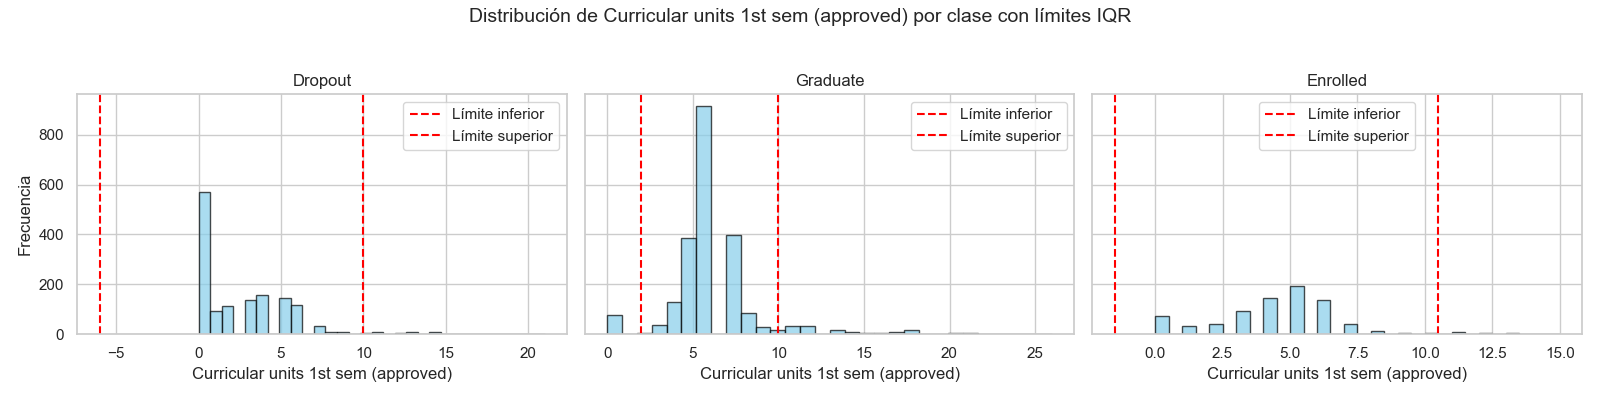
\includegraphics[width=\linewidth]{distribution/Curricular units 1st sem (approved)_distribution.png}
    \caption{Approved}\label{fig:approved1}
  \end{subfigure}\hfill
  \begin{subfigure}[b]{.32\linewidth}
    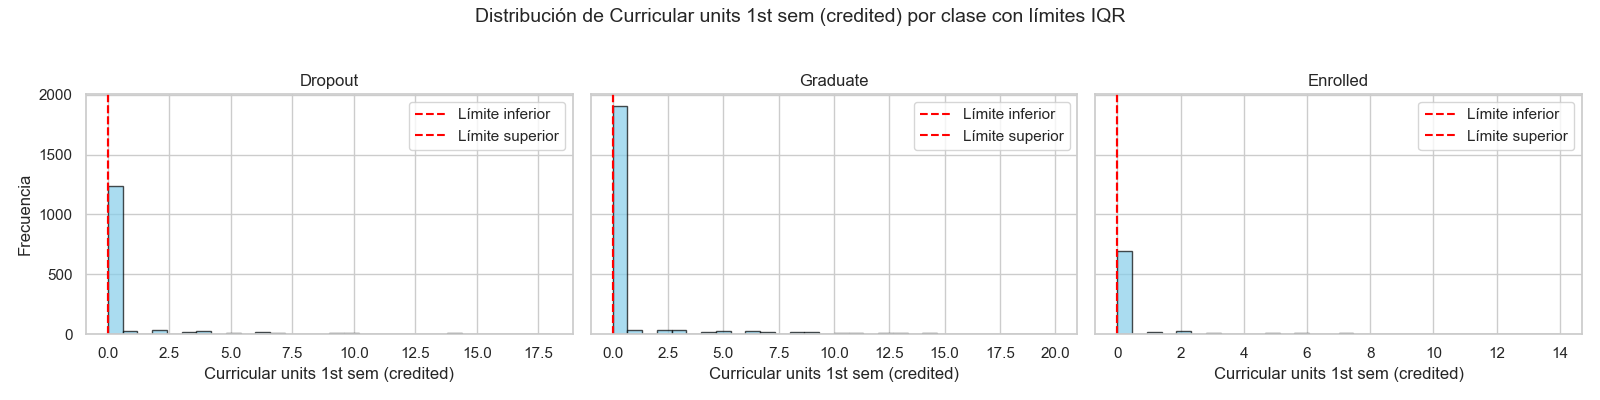
\includegraphics[width=\linewidth]{distribution/Curricular units 1st sem (credited)_distribution.png}
    \caption{Credited}\label{fig:credited1}
  \end{subfigure}\hfill
  \begin{subfigure}[b]{.32\linewidth}
    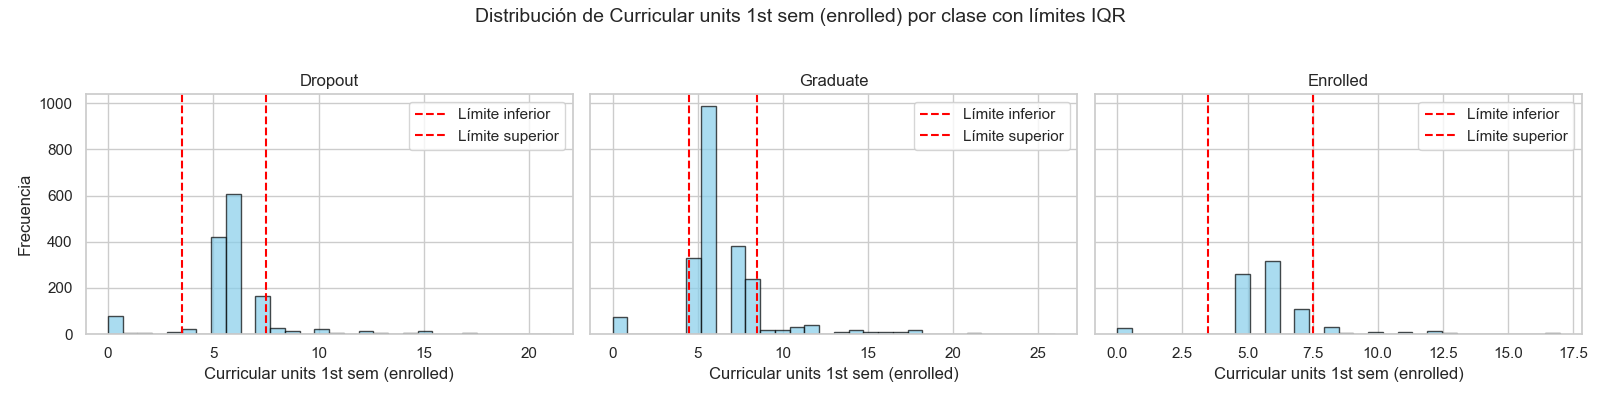
\includegraphics[width=\linewidth]{distribution/Curricular units 1st sem (enrolled)_distribution.png}
    \caption{Enrolled}\label{fig:enrolled1}
  \end{subfigure}

  \medskip  % Salto vertical opcional

  % -------- Fila 2
  \begin{subfigure}[b]{.32\linewidth}
    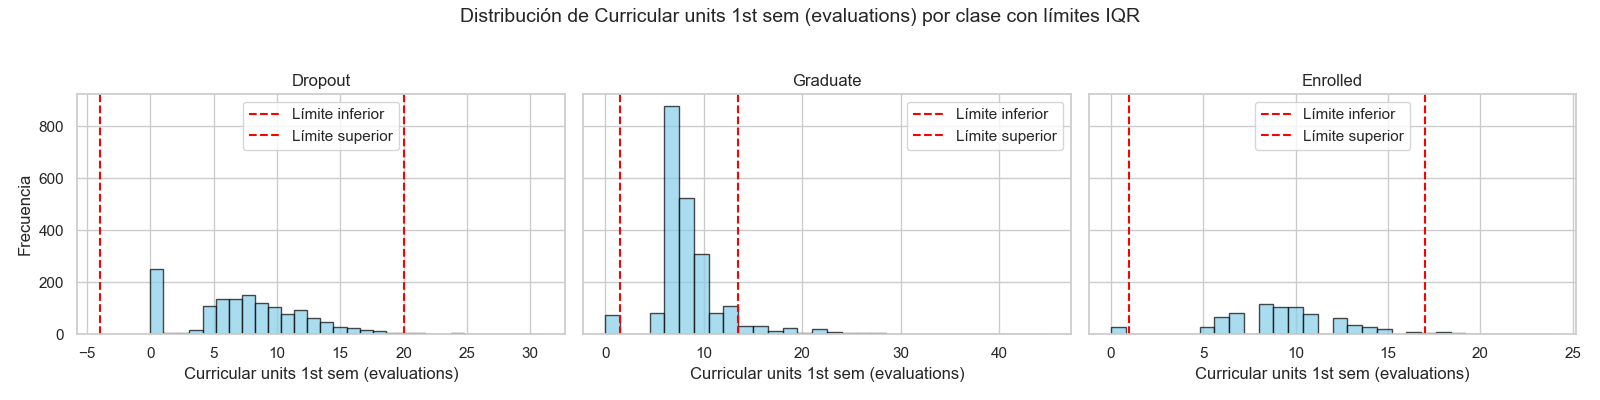
\includegraphics[width=\linewidth]{distribution/Curricular units 1st sem (evaluations)_distribution.png}
    \caption{Evaluations}\label{fig:evaluations1}
  \end{subfigure}\hfill
  \begin{subfigure}[b]{.32\linewidth}
    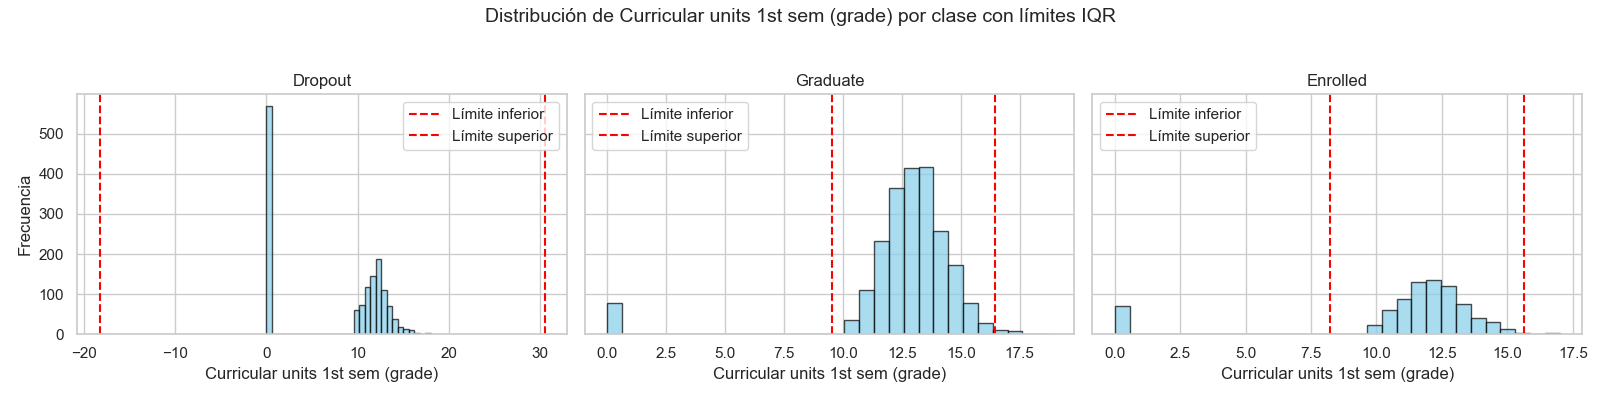
\includegraphics[width=\linewidth]{distribution/Curricular units 1st sem (grade)_distribution.png}
    \caption{Grade}\label{fig:grade1}
  \end{subfigure}\hfill
  \begin{subfigure}[b]{.32\linewidth}
    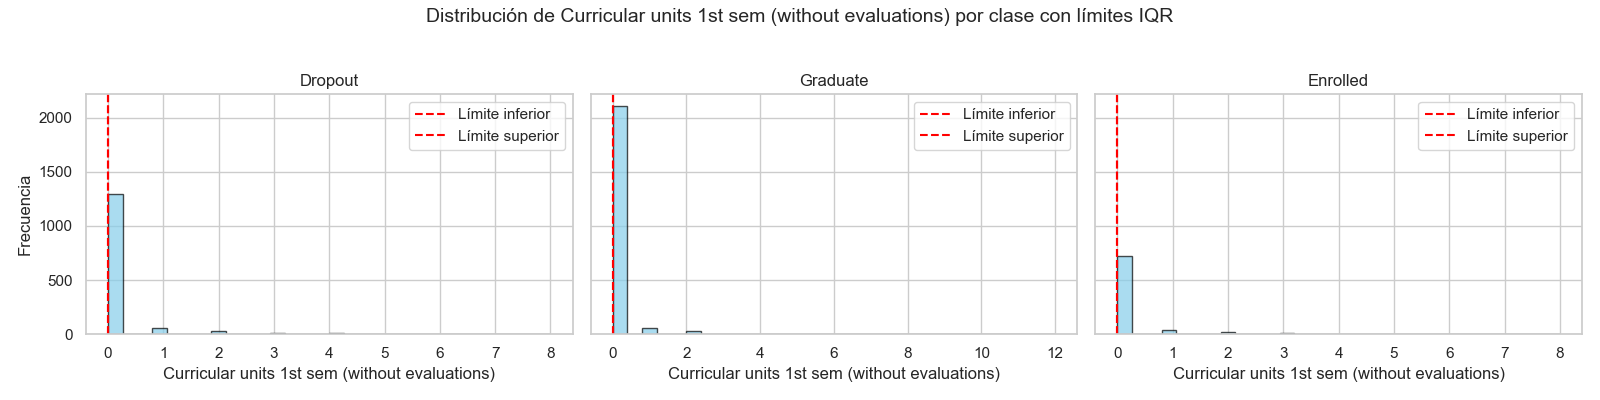
\includegraphics[width=\linewidth]{distribution/Curricular units 1st sem (without evaluations)_distribution.png}
    \caption{Without eval.}\label{fig:witheval1}
  \end{subfigure}

  \caption{Distribuciones por clase de los seis indicadores curriculares del primer semestre.}
  \label{fig:curricular-1s}
\end{figure}


\FloatBarrier
El grupo de figuras \ref{fig:curricular-1s}  resume las distribuciones de seis indicadores de rendimiento.  A continuación se discute cada variable, enfatizando su relación con la variable objetivo.

\begin{itemize}
%----------------------------------------- Approved
\item \textit{Curricular units 1st sem (approved)}  Presenta una asimetría positiva en \textit{Graduate} (mediana $\sim6$) y un pico en $0$ para \textit{Dropout}.  Los valores $>10$ (\emph{high achievers}) son pocos pero significativos
%----------------------------------------- Credited
\item \textit{Curricular units 1st sem (credited)}  Distribución dominada por el valor $0$ en las tres clases.  Los atípicos ($>10$) obedecen a reconocimientos de créditos externos; si se descartasen, se subestimaría la probabilidad de graduación acelerada.
%----------------------------------------- Enrolled
\item \textit{Curricular units 1st sem (enrolled)}  Exhibe colas largas.  El percentil $95$ supera las $10$ matrículas en \textit{Dropout}, lo cual puede ser un indicion que la sobrecarga académica puede aumentar la tasa de abandono.
%----------------------------------------- Evaluations
\item \textit{Curricular units 1st sem (evaluations)}  El 70\% de los alumnos que abandonan registra $0$ evaluaciones, mientras que en \textit{Graduate} el percentil $75$ alcanza $9$ mientras que el percentil $75$ de \textit{Dropout} alcanza 11. Por lo tanto, eliminar los outliners podría redcuir la sensibilidad del modelo de detectar patrones de compromiso y esfuerzo contante frente a retos académico, dados que dichos valores contienen información relevante sobre la conducta de los estudiantes.
%----------------------------------------- Without evaluations
\item \textit{Curricular units 1st sem (without evaluations)}  El valor modal $0$ domina, pero los registros $1$--$2$ indican convalidaciones administrativas; eliminarlos impediría modelar itinerarios curriculares no tradicionales. Mantener estos datos permite una mejor compresión de la diversidad de las trayectorias académicas.
\end{itemize}

%-------------------------------------------------------------------------------
% 2. Variables de progreso curricular – Segundo semestre
%-------------------------------------------------------------------------------
\textbf{Variables curriculares del segundo semestre} \\
\begin{figure}[htbp]
  \centering
  % -------- Fila 1
  \begin{subfigure}[b]{.32\linewidth}
    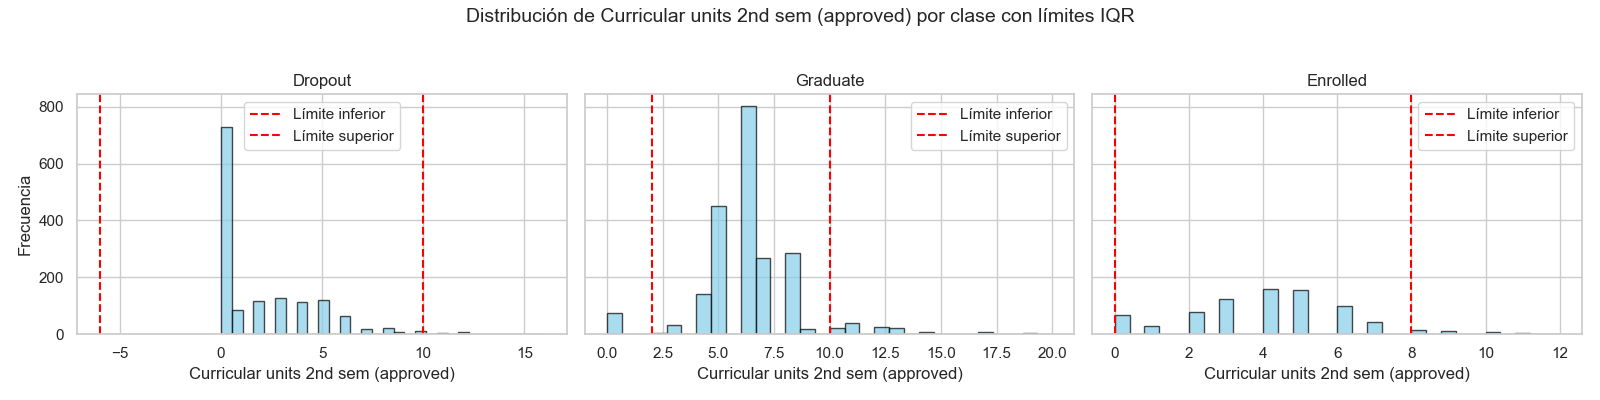
\includegraphics[width=\linewidth]{distribution/Curricular units 2nd sem (approved)_distribution.png}
    \caption{Approved}\label{fig:approved2}
  \end{subfigure}\hfill
  \begin{subfigure}[b]{.32\linewidth}
    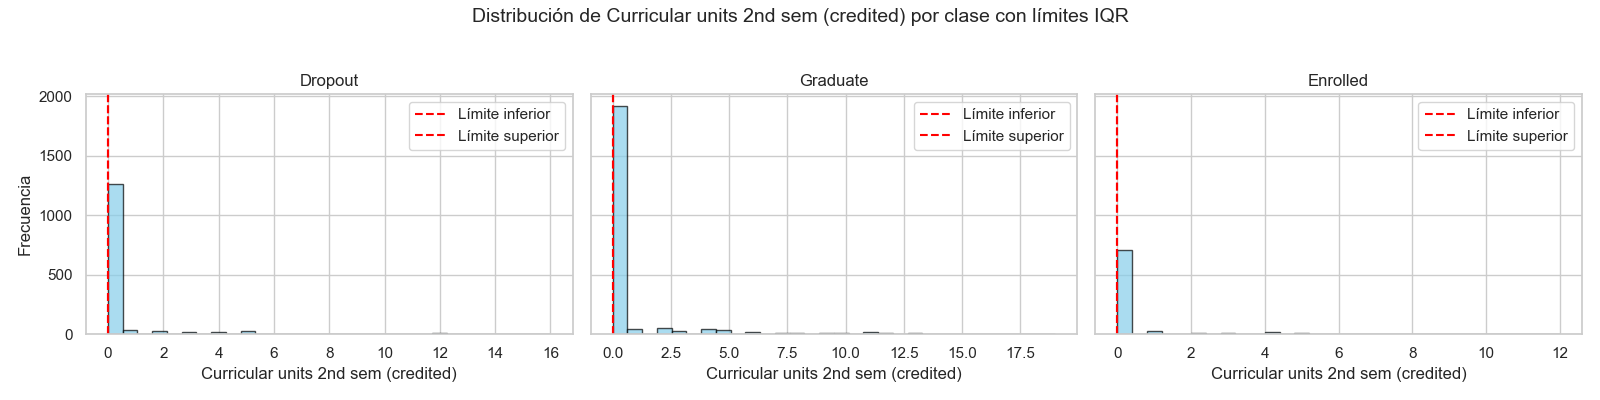
\includegraphics[width=\linewidth]{distribution/Curricular units 2nd sem (credited)_distribution.png}
    \caption{Credited}\label{fig:credited2}
  \end{subfigure}\hfill
  \begin{subfigure}[b]{.32\linewidth}
    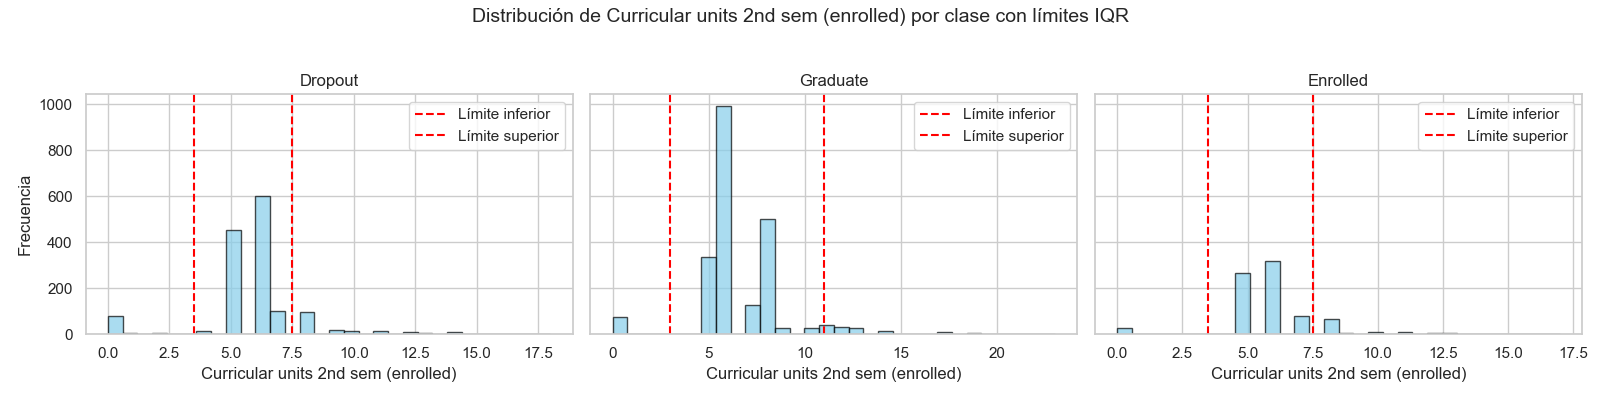
\includegraphics[width=\linewidth]{distribution/Curricular units 2nd sem (enrolled)_distribution.png}
    \caption{Enrolled}\label{fig:enrolled2}
  \end{subfigure}

  \medskip  % Salto vertical opcional

  % -------- Fila 2
  \begin{subfigure}[b]{.32\linewidth}
    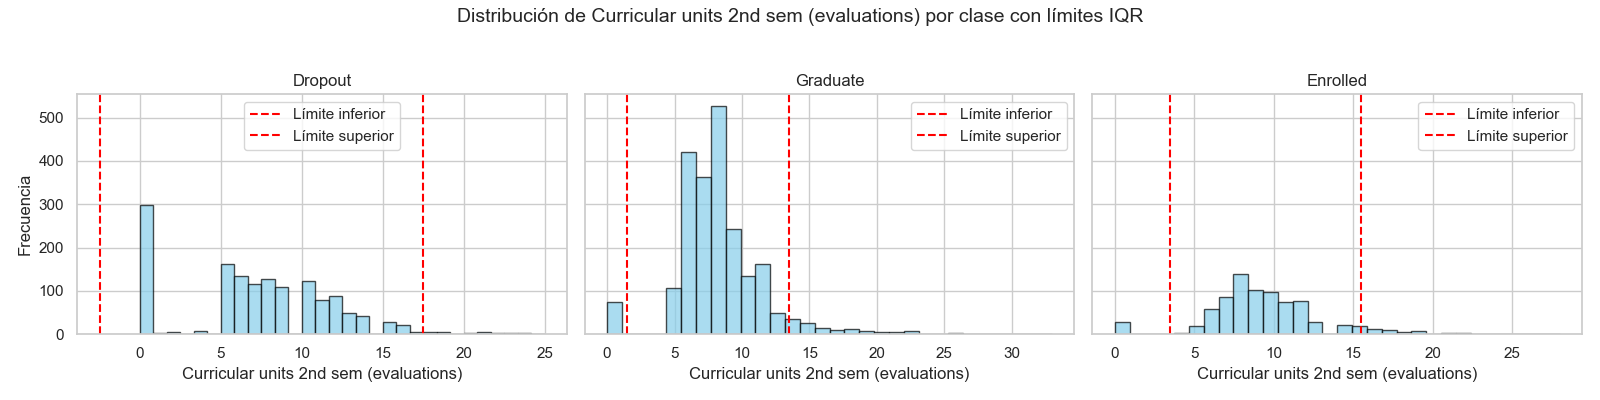
\includegraphics[width=\linewidth]{distribution/Curricular units 2nd sem (evaluations)_distribution.png}
    \caption{Evaluations}\label{fig:evaluations2}
  \end{subfigure}\hfill
  \begin{subfigure}[b]{.32\linewidth}
    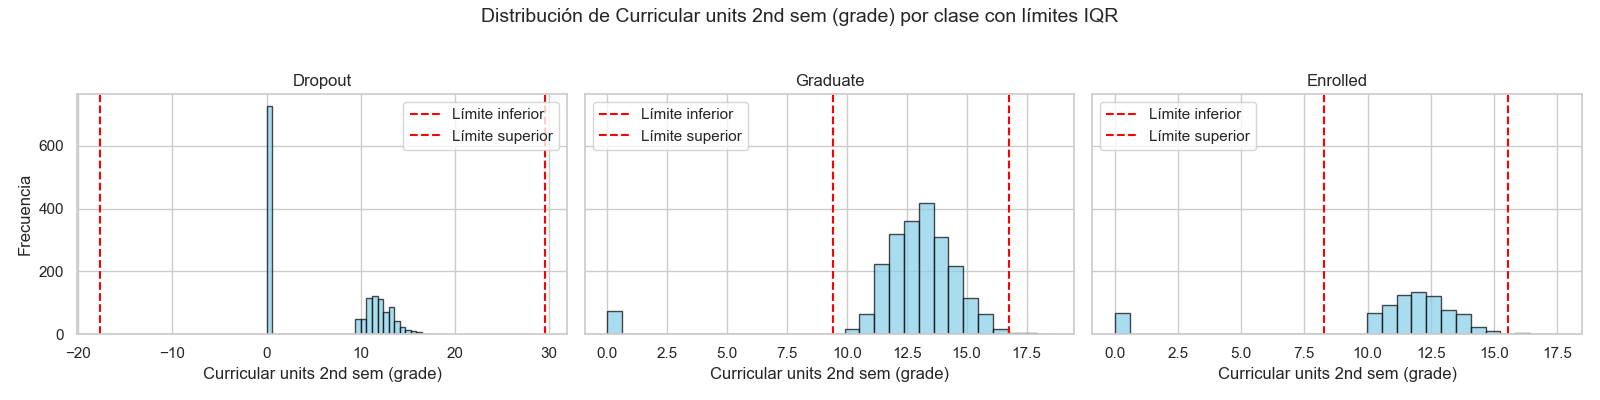
\includegraphics[width=\linewidth]{distribution/Curricular units 2nd sem (grade)_distribution.png}
    \caption{Grade}\label{fig:grade2}
  \end{subfigure}\hfill
  \begin{subfigure}[b]{.32\linewidth}
    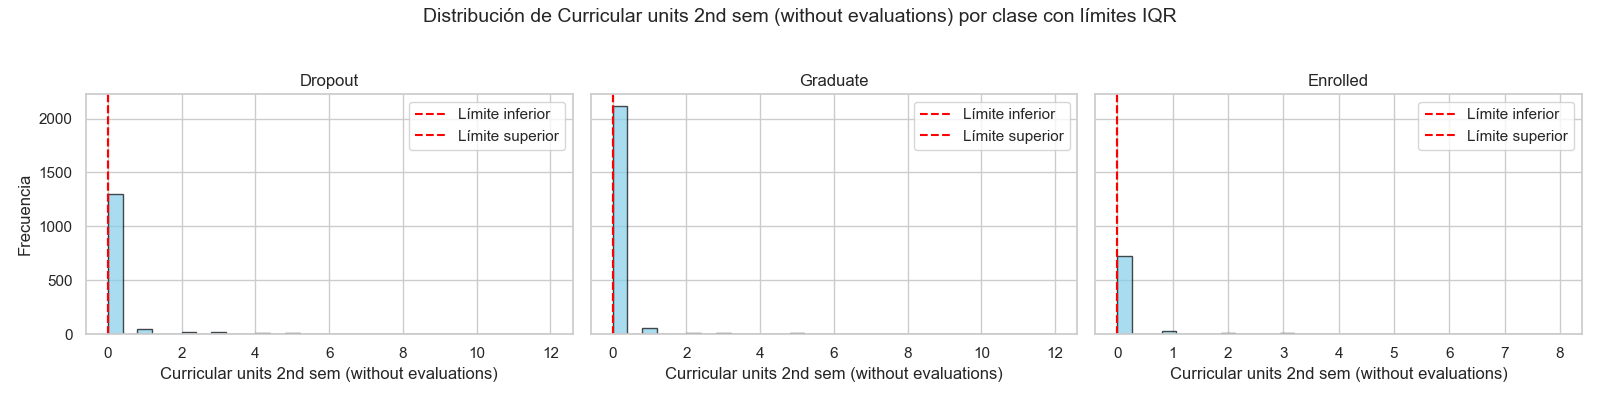
\includegraphics[width=\linewidth]{distribution/Curricular units 2nd sem (without evaluations)_distribution.png}
    \caption{Without eval.}\label{fig:witheval2}
  \end{subfigure}

  \caption{Distribuciones por clase de los seis indicadores curriculares del primer semestre.}
  \label{fig:curricular-2s}
\end{figure}


\FloatBarrier
Los patrones se reproducen con ligeras variaciones (Figura~\ref{fig:curricular-2s}).  Dos hallazgos merecen mención específica:
\begin{enumerate}[label=(\alph*)]
\item En \textit{Curricular units 2nd sem (evaluations)}, los valores $>15$ en \textit{Graduate} se asocian a adelantamiento de asignaturas finales; su exclusión deterioraría la precisión para predecir graduación temprana.
\item \textit{Curricular units 2nd sem (grade)} La mayoría de los datos de la clase \textit{Dropout} son cero, lo que tiene sentido, ya un estudiante que tiene una media muy baja tiene un mayor riesgo de abandonar. Sin embargo, se tienen datos de alumnos que se graduan con notas más altas que la mayoría, por lo que su eliminación implica no tener en cuenta las personas con buena media para la clase \textit{Graduate}.
\end{enumerate}

\paragraph{Síntesis de las variables curriculares.}  Los outliers encapsulan tanto rendimientos excepcionales como situaciones de alto riesgo.  Preservarlos mejora la fidelidad del modelo a la heterogeneidad real del estudiantado.
\section{Las estrategias de codificación aplicadas a variables categóricas}
En Aprendizaje Automático, los modelos no pueden procesar directamente variables categóricas, ya que requieren que todos los atributos sean numéricos. Por tanto, es fundamental transformar las variables categóricas en representaciones que conserven la información semántica sin introducir sesgos artificiales. Este proceso se conoce como codificación de variables categóricas.

Según la teoría estudiada, existen diferentes técnicas de codificación, cuya elección depende principalmente de la \textbf{cardinalidad de la variable} (es decir, el número de categorías únicas) y del tipo de modelo que se vaya a utilizar.

En primer lugar, los variables categoricas binarias tales como `\textbf{\textit{'Gender', 'Scholarship holder', 'Debtor', 'Displaced', 'Educational special needs','Tuition fees up to date','International' }} no necesitan transformación adicional.  Al evaluar sus valores, se llagan a las siguientes conclusiones iniciales:
\begin{itemize}
    \item La distribución entre generación esta razonadamente equilibrado ($65\%$ vs $35\%$) 
    \item Aproximadamente el $25\%$ de los estudiantes poseen beca, lo que puede estar asociado con mayor retención académica o éxito por apoyo económico.
    \item Solo $11\%$ de los estudiantes tienen deudas, esto indica que la clase está un poco desbalanceada.
    \item La variable de \textbf{Tuition fees up to date} es una variable relevante por el contexto económico y tiene potencial como predictor de abandono. El $11.9\%$ de los estudiantes no están al día con las tasas de matrícula.
    \item  La clase internacional, indica que únicamente el $2.5\%$ es de fuera de Portugal, por lo que aunque esta bien codificada, su impacto es mínimo, por lo que se descartará, ya que más adelante se tendrá una variable llamada \textit{is\_foreign}, derivada de la agrupación de las clases de la variable \textit{Nationality}, que medirá lo mismo. De la misma manera, se descartará la variable \textit{Education special needs}, debido a su fuerte desbalance y poca variabilidad, por lo que no se considera relevante por el estudio, en un primer momento.
\end{itemize}

A continuación, se dispondrá al tratamiento de datos categóricos no binarios. Dentro de esta categoría, se tienen más de 8 variables, las cuales tienen entre 6 a 40 clases. Siguiendo la teoría dado en la asignatura, y viendo que se aplicará en la mayoría de los casos, agrupación de valores poco frecuentes y luego one-hot enconding.

\subsection*{Maritial Status}
\begin{table}[H]
\centering
\begin{tabular}{|c|l|c|c|}
\hline
\textbf{Código} & \textbf{Categoría} & \textbf{Frecuencia} & \textbf{Proporción (\%)} \\
\hline
1 & Soltero/a (Single)              & 3919 & 88.59 \\
2 & Casado/a (Married)             & 379  & 8.57 \\
4 & Divorciado/a (Divorced)        & 91   & 2.06 \\
5 & Unión de hecho (Facto union)   & 25   & 0.57 \\
6 & Separado/a legalmente          & 6    & 0.14 \\
3 & Viudo/a (Widower)              & 4    & 0.09 \\
\hline
\end{tabular}
\caption{Distribución original de la variable \textit{Marital Status}}
\label{tab:marital-status}
\end{table}

Se observa que la mayoría de los estudiantes está solteros, y que existen varias clases con pocos datos, menos del $1\%$ de los datos, por lo que se opta a agruparlos en una sola clase, para evitar ruido en la muestra:
\begin{table}[H]
    \centering
    \begin{tabular}{|c|l|c|c|}
        \hline
        \textbf{Código} & \textbf{Categoría} & \textbf{Frecuencia} & \textbf{Proporción (\%)} \\
        \hline
        1 & Single     & 3919 & 88.59 \\
        2 & Married    & 379  & 8.57 \\
        4 & Divorced   & 91   & 2.06 \\
        0 & Other (3, 5, 6) & 35   & 0.79 \\
        \hline
    \end{tabular}
    \caption{Distribución agrupada de \textit{Marital Status}}
    \label{tab:marital-status-new}
\end{table}
A continuación, dada la nueva distribución de la variable, se procede a aplicar la codificación \textit{One-Hot}. Esta técnica consiste en generar un vector binario para cada categoría posible del atributo, de modo que exactamente una posición toma el valor $1$ y las demás $0$. Esta codificación ha sido seleccionada por la baja cardinalidad del atributo, lo que la hace eficiente y adecuada. Como resultado, se han creado cuatro nuevas columnas en el conjunto de datos, cada una representando una de las categorías originales de la variable.

\subsection*{Variable: Father's Occupation}
Se tienen 46 categorías de este variable, por lo que no se puede aplicar directamente one-hot enconder, ya que resulta en un uso ineficiente de la memoria. Por lo que se calcula cuán de balanceada se encuentra esta variable, y se halla que existen 34 categorías cuya representación es menor al $1\%$, por lo que se opta por agrupar dichas categorías en una sola, por lo que la nueva distribución de esta variable sería de la siguiente forma:
\begin{table}[H]
    \centering
    \begin{tabular}{|c|l|c|c|}
        \hline
        \textbf{Código} & \textbf{Categoría} & \textbf{Frecuencia} & \textbf{Proporción} \\
        \hline
        9  & Unskilled Workers & 1010 & 0.2283 \\
        7  & Skilled Industry  & 666  & 0.1505 \\
        5  & Services/Sellers  & 516  & 0.1166 \\
        4  & Admin Staff       & 386  & 0.0873 \\
        3  & Technicians       & 384  & 0.0868 \\
        8  & Machine Operators & 318  & 0.0719 \\
        10 & Armed Forces      & 266  & 0.0601 \\
        6  & Agriculture       & 242  & 0.0547 \\
        2  & Scientific Spec.  & 197  & 0.0445 \\
        -1 & Otros/OOV         & 177  & 0.0400 \\
        1  & Executives        & 134  & 0.0303 \\
        0  & Student           & 128  & 0.0289 \\
        \hline
    \end{tabular}
    \caption{Distribución agrupada de \textit{Father's occupation}}
    \label{tab:father_occ}
\end{table}
Una vez identificadas las variables categóricas de alta cardinalidad, se procede a aplicar una estrategia de agrupación seguida de codificación \textit{One-Hot}, con el objetivo de reducir la dimensionalidad y evitar una representación dispersa que pueda perjudicar el rendimiento de algunos modelos.
\\

A continuación se resumen los criterios de transformación empleados:

\begin{itemize}
    \item \textbf{\textit{Mother's occupation}}: Presenta 32 categorías originales. Se detecta que 26 ocupaciones representan menos del $5\%$ de los datos cada una. Estas se agrupan en una única categoría denominada \textit{Other}, reduciendo la cardinalidad a 7 clases antes de aplicar \textit{One-Hot}.
    \begin{table}[H]
    \centering
    \begin{tabular}{|c|l|c|}
        \hline
        \textbf{Código} & \textbf{Categoría} & \textbf{Proporción} \\
        \hline
        9  & Unskilled Workers     & 0.356 \\
        4  & Admin Staff           & 0.185 \\
        -1 & Otros/OOV             & 0.126 \\
        5  & Services/Sellers      & 0.120 \\
        3  & Technicians           & 0.079 \\
        2  & Scientific Specialists & 0.072 \\
        7  & Skilled Industry      & 0.061 \\
        \hline
    \end{tabular}
    \caption{Distribución agrupada de \textit{Mother's occupation}}
    \label{tab:mother_occ}
    \end{table}
    
    \item \textbf{\textit{Application mode}}: Cuenta con 18 categorías iniciales. Nueve de ellas tienen una frecuencia inferior al $1\%$, por lo que se agrupan en una sola categoría residual. Tras esta transformación, se trabaja con 10 clases.
    \begin{table}[H]
    \centering
    \begin{tabular}{|c|l|c|}
        \hline
        \textbf{Código} & \textbf{Categoría} & \textbf{Proporción} \\
        \hline
        1 & General (1st phase) & 0.3861 \\
        17 & General (2nd phase) & 0.1971 \\
        39 & Over 23 years old & 0.1774 \\
        43 & Change of course & 0.0705 \\
        44 & Technological diploma & 0.0481 \\
        7 & Other higher ed. & 0.0314 \\
        -1 & Other/OOV & 0.0305 \\
        18 & General (3rd phase) & 0.0280 \\
        42 & Transfer & 0.0174 \\
        51 & Change institution/course & 0.0133 \\
        \hline
    \end{tabular}
    \caption{Distribución agrupada de \textit{Application mode}}
    \label{tab:application_mode}
    \end{table}
    \item \textbf{\textit{Application order}}: Tiene 8 valores posibles que representan el orden de preferencia en la solicitud. Dado que estos valores tienen significado ordinal, no se agrupan ni se transforman, manteniéndose como variable numérica discreta.
    
    \item \textbf{\textit{Course}}: Con 17 códigos distintos de asignaturas, esta variable se conserva tal cual, ya que cada código representa una titulación específica, y su agrupación implicaría pérdida de información relevante para el modelo.
    \begin{table}[H]
    \centering
    \begin{tabular}{|c|l|c|}
        \hline
        \textbf{Código} & \textbf{Curso} & \textbf{Proporción} \\
        \hline
        9500 & Nursing                             & 0.173 \\
        9147 & Management                          & 0.086 \\
        9238 & Social Service                      & 0.080 \\
        9085 & Veterinary Nursing                  & 0.076 \\
        9773 & Journalism and Communication        & 0.075 \\
        9670 & Advertising and Marketing Management & 0.061 \\
        9991 & Management (evening attendance)     & 0.0605 \\
        9254 & Tourism                             & 0.057 \\
        8014 & Social Service (evening attendance) & 0.0569 \\
        171  & Animation and Multimedia Design     & 0.049 \\
        9003 & Agronomy                            & 0.047 \\
        9853 & Basic Education                     & 0.043 \\
        9119 & Informatics Engineering             & 0.038 \\
        9130 & Equinculture                        & 0.0318 \\
        9556 & Oral Hygiene                        &  0.0194\\
        9070 & Communication Design                & 0.0510 \\
        33   & Biofuel Production Technologies     & 0.0027 \\
        \hline
    \end{tabular}
    \caption{Distribución agrupada de \textit{Course grouped}}
    \label{tab:course_grouped}
\end{table}
    \item \textbf{\textit{Previous qualification}}: Inicialmente con 17 categorías, de las cuales 12 tienen una frecuencia menor al $1\%$. Se agrupan en una clase residual, lo que permite reducir el número total de categorías antes de la codificación.
    \begin{table}[H]
    \centering
    \begin{tabular}{|c|l|c|}
        \hline
        \textbf{Código} & \textbf{Categoría} & \textbf{Proporción} \\
        \hline
        1 & Secondary education & 0.8402 \\
        39 & Techn. specialization & 0.0495 \\
        -1 & Other/OOV & 0.0452 \\
        19 & Basic ed. 3rd cycle & 0.0366 \\
        3 & Higher education & 0.0285 \\
        \hline
    \end{tabular}
    \caption{Distribución agrupada de \textit{Previous qualification}}
    \label{tab:previous_qualification}
    \end{table}

    \item \textbf{\textit{Nationality}}: De sus 21 categorías originales, más del $97\%$ de los estudiantes pertenecen a la nacionalidad local. Por ello, se simplifica esta variable a una codificación binaria denominada \texttt{is\_foreign}, donde 0 indica nacionalidad local y 1 corresponde a extranjero.
    
    \item \textbf{\textit{Mother's qualification}}: De las 29 categorías originales, se agrupa por nivel educativo y se reducen a 6 clases antes de aplicar la codificación.
    \begin{table}[H]
    \centering
    \begin{tabular}{|c|l|c|}
        \hline
        \textbf{Código} & \textbf{Categoría} & \textbf{Proporción} \\
        \hline
        1 & Secondary education & 0.2416 \\
        37 & Basic ed. 3rd cycle & 0.2281 \\
        19 & Higher education & 0.2154 \\
        4 & Basic ed. 2nd cycle & 0.1288 \\
        38 & Basic ed. 1st cycle & 0.1270 \\
        -1 & Other/OOV & 0.0590 \\
        \hline
    \end{tabular}
    \caption{Distribución agrupada de \textit{Mother's qualification}}
    \label{tab:mothers_qualification}
    \end{table}

    \item \textbf{\textit{Father's qualification}}: Siguiendo el mismo criterio que la anterior, pasa de 34 a 6 categorías tras la agrupación.
    \begin{table}[H]
    \centering
    \begin{tabular}{|c|l|c|}
        \hline
        \textbf{Código} & \textbf{Categoría} & \textbf{Proporción} \\
        \hline
        37 & Basic ed. 3rd cycle & 0.2733 \\
        19 & Higher education & 0.2188 \\
        1 & Secondary education & 0.2043 \\
        38 & Basic ed. 1st cycle & 0.1587 \\
        4 & Basic ed. 2nd cycle & 0.0791 \\
        -1 & Other/OOV & 0.0658 \\
        \hline
    \end{tabular}
    \caption{Distribución agrupada de \textit{Father's qualification}}
    \label{tab:fathers_qualification}
    \end{table}
\end{itemize}

\section{La distribución de la variable objetivo (Target) y el desbalance de clases}
\label{sec:target-balance}

\subsection{Análisis inicial de la variable \texttt{Target}}

La variable objetivo \texttt{Target} es de tipo categórico con tres posibles clases: \texttt{Graduate}, \texttt{Dropout} y \texttt{Enrolled}. La distribución de los datos antes del preprocesamiento es la siguiente:

\begin{itemize}
    \item \texttt{Graduate}: 49.93\% de los datos.
    \item \texttt{Dropout}: 32.12\% de los datos.
    \item \texttt{Enrolled}: 17.95\% de los datos.
\end{itemize}

Esta distribución evidencia un cierto desbalance de clases, particularmente en la clase \texttt{Enrolled}, que representa menos de una quinta parte del total. Aunque no se trata de un caso extremo, este desequilibrio puede inducir sesgos en los modelos de aprendizaje automático supervisado, especialmente aquellos sensibles a la proporción de clases (como la regresión logística o k-NN). Este tipo de problemas puede generar:

\begin{itemize}
    \item Pérdida de capacidad predictiva en las clases minoritarias.
    \item Modelos con alta precisión general pero bajo \textit{recall} en clases subrepresentadas.
    \item Umbrales de clasificación que no son óptimos para todas las clases.
\end{itemize}
\subsection{La justificación y aplicación de técnicas de rebalanceo como SMOTE.}
Para abordar este desequilibrio y asegurar un aprendizaje más equitativo entre clases, se optó por aplicar la técnica de sobre-muestreo \textbf{SMOTE (Synthetic Minority Over-sampling Technique)}. Esta técnica genera ejemplos sintéticos de las clases minoritarias interpolando entre ejemplos reales cercanos en el espacio de características.

Se utilizó la clase \texttt{SMOTE} de la biblioteca \texttt{imblearn}, con una estrategia específica de muestreo para cada clase, lo que permite mantener una distribución balanceada pero realista:

\begin{lstlisting}[language=Python]
from sklearn.preprocessing import LabelEncoder
from imblearn.over_sampling import SMOTE

le = LabelEncoder()
X_encoded = df9.drop(columns=['Target'])
y_multi = le.fit_transform(df9['Target'])  # Dropout=0, Enrolled=1, Graduate=2 

sm = SMOTE(sampling_strategy={0: 2200, 1: 2000, 2: 2500}, random_state=42)
X_resampled, y_resampled = sm.fit_resample(X_encoded, y_multi)
\end{lstlisting}

\subsection{Detalles del procedimiento}

\begin{itemize}
    \item Se codificó la variable \texttt{Target} con \texttt{LabelEncoder}, asignando los valores:
    \begin{itemize}
        \item \texttt{Dropout}: 0
        \item \texttt{Enrolled}: 1
        \item \texttt{Graduate}: 2
    \end{itemize}
    \item Se aplicó \texttt{SMOTE} únicamente a las variables ya preprocesadas (numéricas y categóricas codificadas).
    \item Se generaron 1,000 ejemplos sintéticos para la clase \texttt{Enrolled} y se aumentaron las clases \texttt{Dropout} y \texttt{Graduate} a 2,200 y 2,500 muestras respectivamente.
    \item El procedimiento preserva la estructura del dataset original y no introduce ruido aleatorio, ya que los ejemplos generados están basados en vecinos reales.
\end{itemize}

\subsection{Estado final tras SMOTE}

La nueva distribución de clases después del rebalanceo es:

\begin{itemize}
    \item \texttt{Graduate}: 2,500 ejemplos.
    \item \texttt{Dropout}: 2,200 ejemplos.
    \item \texttt{Enrolled}: 2,000 ejemplos.
\end{itemize}

Esta proporción permite mantener una ligera preponderancia de la clase \texttt{Graduate} (coherente con la distribución original), sin sacrificar el rendimiento predictivo sobre las clases minoritarias.

Tras estos análisis exhasutivo de los datos, el dataset ya está listo para poder crear modelos e inferir sobre ellos.
\chapter{Modelo K-Vecinos más Cercanos (K-NN)}

En este apartado se desarrolla la implementación del modelo \textit{K-Vecinos más Cercanos} (K-Nearest Neighbors, K-NN), cuyo enfoque se basa en la idea de que las observaciones similares tienden a compartir la misma clase. El modelo predice el destino académico de un estudiante —abandono (\textit{Dropout}), inscripción activa (\textit{Enrolled}) o graduación (\textit{Graduate})— comparando sus características con las de los estudiantes más cercanos en el conjunto de entrenamiento.

A diferencia de modelos como la regresión logística o redes neuronales, K-NN no realiza un aprendizaje explícito durante el entrenamiento. En su lugar, almacena el conjunto de entrenamiento y, cuando se presenta un nuevo caso, busca los \textit{k} ejemplos más próximos utilizando una métrica de distancia (en este caso, la distancia euclídea). La clase asignada es la más frecuente entre estos \textit{k} vecinos.

\section*{Selección del valor óptimo de \textit{k}}

La elección del número de vecinos \textit{k} es crítica para el rendimiento del modelo. Para ello, se diseñó un algoritmo que prueba múltiples valores de \textit{k}, evaluando la \textit{accuracy} en el conjunto de test para cada uno. El valor que maximiza esta métrica se selecciona como óptimo. En este caso, el mejor rendimiento se obtuvo con \textbf{k = 1}, alcanzando una \textit{accuracy} del \textbf{77\,\%} sobre el conjunto de test.

\begin{figure}
    \centering
    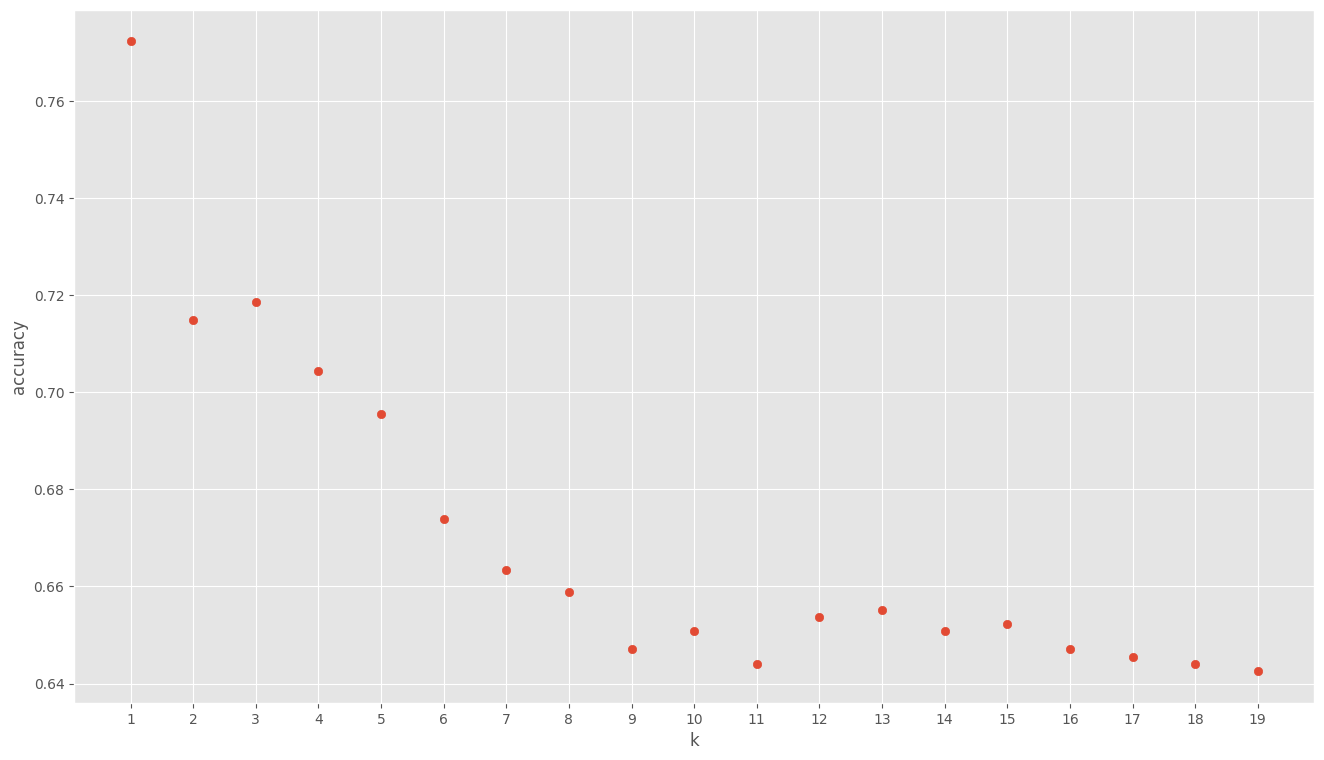
\includegraphics[width=0.68\linewidth]{mejor k.png}
    \caption{Gráfico que muestra la precisión del modelo con K del 1 al 20}
    \label{fig:boxplot-age}
\end{figure}

Este valor indica que, para este conjunto de datos y tras el preprocesamiento realizado, el ejemplo más cercano es suficientemente representativo como para realizar predicciones fiables, sin necesidad de considerar múltiples vecinos.

\newpage
\section*{Evaluación del rendimiento}

Con \textit{k = 1}, el modelo mostró una precisión del \textbf{100\,\%} sobre el conjunto de entrenamiento, lo cual es esperable debido a que un modelo con \textit{k = 1} clasifica cada punto del entrenamiento comparándolo consigo mismo (distancia cero). Esta característica implica un riesgo potencial de sobreajuste (\textit{overfitting}), aunque en este caso el rendimiento en el test (77\,\%) sugiere que el modelo generaliza razonablemente bien.

La matriz de confusión obtenida fue la siguiente:

\[
\begin{bmatrix}
334 & 54 & 54 \\
11 & 365 & 28 \\
49 & 109 & 336 \\
\end{bmatrix}
\]

Donde:

\begin{itemize}
  \item La clase 0 (\textit{Dropout}) tuvo 442 casos reales, de los cuales 334 fueron correctamente clasificados. Se confundieron 54 con \textit{Enrolled} y 54 con \textit{Graduate}.
  \item La clase 1 (\textit{Enrolled}) tuvo 404 casos reales, con 365 clasificaciones correctas. Se confundieron 11 con \textit{Dropout} y 28 con \textit{Graduate}.
  \item La clase 2 (\textit{Graduate}) tuvo 494 casos reales, con 336 clasificaciones correctas. Se confundieron 49 con \textit{Dropout} y 109 con \textit{Enrolled}.
\end{itemize}

Las métricas de evaluación permiten analizar el rendimiento del modelo más allá de la precisión global, ofreciendo una visión más detallada sobre cómo se comporta el clasificador en cada una de las clases. Se han calculado tres métricas principales para cada categoría del destino académico:

\begin{itemize}
  \item \textbf{Precision}: mide la proporción de predicciones correctas entre todas las veces que el modelo predijo una clase determinada. Valores altos indican que el modelo comete pocos falsos positivos.
  \begin{itemize}
    \item \textit{Dropout}: 0.85
    \item \textit{Enrolled}: 0.69
    \item \textit{Graduate}: 0.80
  \end{itemize}
  
  \item \textbf{Recall}: representa la capacidad del modelo para identificar correctamente los casos reales de cada clase, es decir, cuántos verdaderos positivos encuentra sobre el total de ejemplos reales. Valores altos indican que el modelo comete pocos falsos negativos.
  \begin{itemize}
    \item \textit{Dropout}: 0.76
    \item \textit{Enrolled}: 0.90
    \item \textit{Graduate}: 0.68
  \end{itemize}
  
  \item \textbf{F1-score}: es la media armónica entre la precisión y el recall, y proporciona una métrica balanceada que resulta especialmente útil cuando hay desbalance entre clases.
  \begin{itemize}
    \item \textit{Dropout}: 0.80
    \item \textit{Enrolled}: 0.78
    \item \textit{Graduate}: 0.74
  \end{itemize}
\end{itemize}

El modelo muestra un comportamiento especialmente destacable en la clase \textit{Enrolled}, con un \textbf{recall del 90\,\%}, lo que indica que es capaz de identificar correctamente a la mayoría de los estudiantes que permanecen inscritos. Sin embargo, su \textbf{precisión en esta clase es más baja (0.69)}, lo que implica que también clasifica erróneamente como inscritos a algunos estudiantes que, en realidad, abandonan o se gradúan.

Por otro lado, en la clase \textit{Dropout} el modelo presenta un equilibrio favorable entre precisión y recall (0.85 y 0.76 respectivamente), lo que sugiere que detecta bien los casos de abandono, con pocos errores tanto por exceso como por omisión.

Finalmente, la clase \textit{Graduate} presenta buena precisión (0.80), pero un \textbf{recall más bajo (0.68)}, lo que significa que aunque cuando predice que alguien se gradúa suele acertar, deja de identificar a varios estudiantes que sí se gradúan realmente.

La precisión global del modelo (\textit{accuracy}) es del \textbf{77\,\%}, es decir, clasifica correctamente aproximadamente 3 de cada 4 estudiantes. La \textbf{media ponderada del F1-score}, que tiene en cuenta el tamaño de cada clase, también es de \textbf{0.77}, lo que confirma un rendimiento sólido y balanceado, incluso frente a la distribución desigual entre clases.


\section*{Predicción de nuevos estudiantes}

El modelo fue utilizado para predecir la probabilidad de destino académico de nuevos estudiantes. A modo de ejemplo, se presentan los resultados para cinco perfiles:

\begin{itemize}
  \item Estudiante 1: 85\,\% de probabilidad de continuar inscrito, 15\,\% de graduarse, 0\,\% de abandonar.
  \item Estudiante 2: Igual distribución que el anterior.
  \item Estudiante 3: 92\,\% de probabilidad de inscripción, 8\,\% de graduación, 0\,\% de abandono.
  \item Estudiante 4: 77\,\% de inscripción, 23\,\% de graduación, 0\,\% de abandono.
  \item Estudiante 5: 69\,\% de inscripción, 23\,\% de graduación, 8\,\% de abandono.
\end{itemize}

Estas predicciones permiten interpretar el modelo más allá de una clasificación directa, aportando una herramienta útil para establecer alertas o intervenciones preventivas en aquellos estudiantes con riesgo elevado de abandono.

\section*{Visualización y variables relevantes}

Para interpretar gráficamente el funcionamiento del modelo, se generó un diagrama de dispersión utilizando dos variables clave: la \textit{nota de admisión} y la \textit{cualificación previa}. Cada punto representa a un estudiante, coloreado según su clase real. Se observó que:

\begin{itemize}
  \item Los estudiantes con mayores notas de admisión se agrupan con mayor frecuencia en la clase \textit{Graduate}.
  \item Los estudiantes con cualificaciones previas más bajas aparecen más frecuentemente en las clases \textit{Dropout} o \textit{Enrolled}.
\end{itemize}

Estas observaciones apoyan la validez del enfoque K-NN y refuerzan la importancia de estas variables en la predicción del destino académico.

\chapter{Análisis Predictivo del Abandono Estudiantil mediante Árboles de Decisión}

\section{Introducción}
En el siguiente apartado se intenta predecir el destino académico de un estudiante, clasificándolo en algunas de los siguientes categorías: \textit{Dropout, Graduated o Enrolled} - mediante el uso y árboles de decisión. El objetivo es diseñar un modelo capaz de identificar con alta fiabilidad a aquellos estudiantes con riesgo de abandono, de modo que se puedan aplicar técnicas de apoyo oportunas.

\section{Metodología}
\subsection{Preparación y división de los datos}
Antes de la implementación del modelo y su posterior interpretación, se definen las variables predictoras \textit{X} y la variable objetivo \textit{y} (codificada como $0=\mathrm{Dropout}$, $1=\mathrm{Enrolled}$, $2=\mathrm{Graduate}$) y se realiza una división estratificada en conjuntos de entrenamiento (80\%) y prueba (20\%), con semilla fija \texttt{random\_state=42} para garantizar la reproducibilidad.
\section{Configuraciñon de los modelos}
Se construyen dos serie de árboles de decisión idénticos en su lógica, peor con distinto \textbf{criterio de división}:
\begin{itemize}
    \item \textbf{Serie A Gini}: \texttt{criterion='gini'}
    \item \textbf{Serie B Entropía}: \texttt{criterion='entropy'}
\end{itemize}
Para ambas series, se instancias los siguientes valores: \texttt{min\_impurity\_decrease=0.001} \footnote{\texttt{min\_impurity\_decrease=0.001} es ampliamente utilizado en la literatura y en la práctica porque ofrece un buen equilibrio entre permitir divisiones útiles y evitar el sobreajuste. Este valor implica que un nodo solo se dividirá si la reducción de impureza entre padre e hijos es al menos 0.001, es decir, si una división mejora la pureza de forma real y significativa, se permite pero en caso contrario, el árbol no divide y mantiene el nodo como hoja. Esto permite divisiones irrelevantes, ramas inútiles que dificultan la interpretación y el riesgo de sobreajuste.} y \texttt{random\_state=42} para garantizar la reproducibilidad
\end{document}


